% chapters/chapter3/3_3_lqr_traj.tex
% !TeX root=../../main.tex

\section{ارزیابی کنترل‌کننده (\lr{LQR}) در ردیابی مسیر}
\label{sec:lqr_traj_analysis}

پدیده‌های مخرب مشاهده‌شده در پاسخ پله (نظیر اشباع عملگرها و ناپایداری آونگ)، لزوم گذار از استراتژی تنظیم‌گر نقطه ثابت (\lr{Set-point Regulation}) به معماری ردیابی مسیر (\lr{Trajectory Tracking}) را اثبات می‌کند. در این رویکرد، پروفایل‌های پیوستهٔ موقعیت، سرعت و شتاب که توسط برنامه‌ریز مسیر تولید شده‌اند، به عنوان مرجع به سیستم اعمال می‌شوند. فرمان کنترلی نهایی در این معماری از جمع جبری سیگنال پیش‌خور تحلیلی (فیدفوروارد) برای غلبه بر اینرسی مسیر، و سیگنال فیدبک \lr{LQR} برای جبران خطای لحظه‌ای و میراسازی نوسانات تشکیل شده است.

\subsection{تحلیل نتایج شبیه‌سازی: جابجایی کوتاه‌برد ($0.5$ متر)}

در سناریوی نخست، کالسکه برای طی کردن مسافت $0.5$ متر تحت هدایت معماری ردیاب قرار گرفت. همان‌طور که در شکل \ref{fig:lqr_traj_x_05} مشاهده می‌شود، سیستم با دقت بسیار بالا و با فراجهش اندک، مسیر مرجع را ردیابی کرده و در حدود ثانیهٔ $2.5$ به نقطهٔ هدف می‌رسد.

بررسی دینامیک نوسان در شکل \ref{fig:lqr_traj_theta_05} حاکی از آن است که بیشینهٔ انحراف آونگ در طول این مانور به حدود $0.1$ رادیان محدود شده است. تفکیک سیگنال‌های کنترلی در شکل \ref{fig:lqr_traj_fs_05} ساختار توزیع تلاش کنترلی را روشن می‌سازد؛ بار اصلی شتاب‌دهی و ترمزگیری کالسکه کاملاً بر عهدهٔ سیگنال فیدفوروارد است و سیگنال فیدبک \lr{LQR} با دامنهٔ محدود خود، صرفاً وظیفهٔ حفظ پایداری، جبران خطای گذرا و میراسازی نرم نوسانات آونگ را به دوش می‌کشد.

\begin{figure}[htbp]
    \centering
    \begin{minipage}{0.48\textwidth}
        \centering
        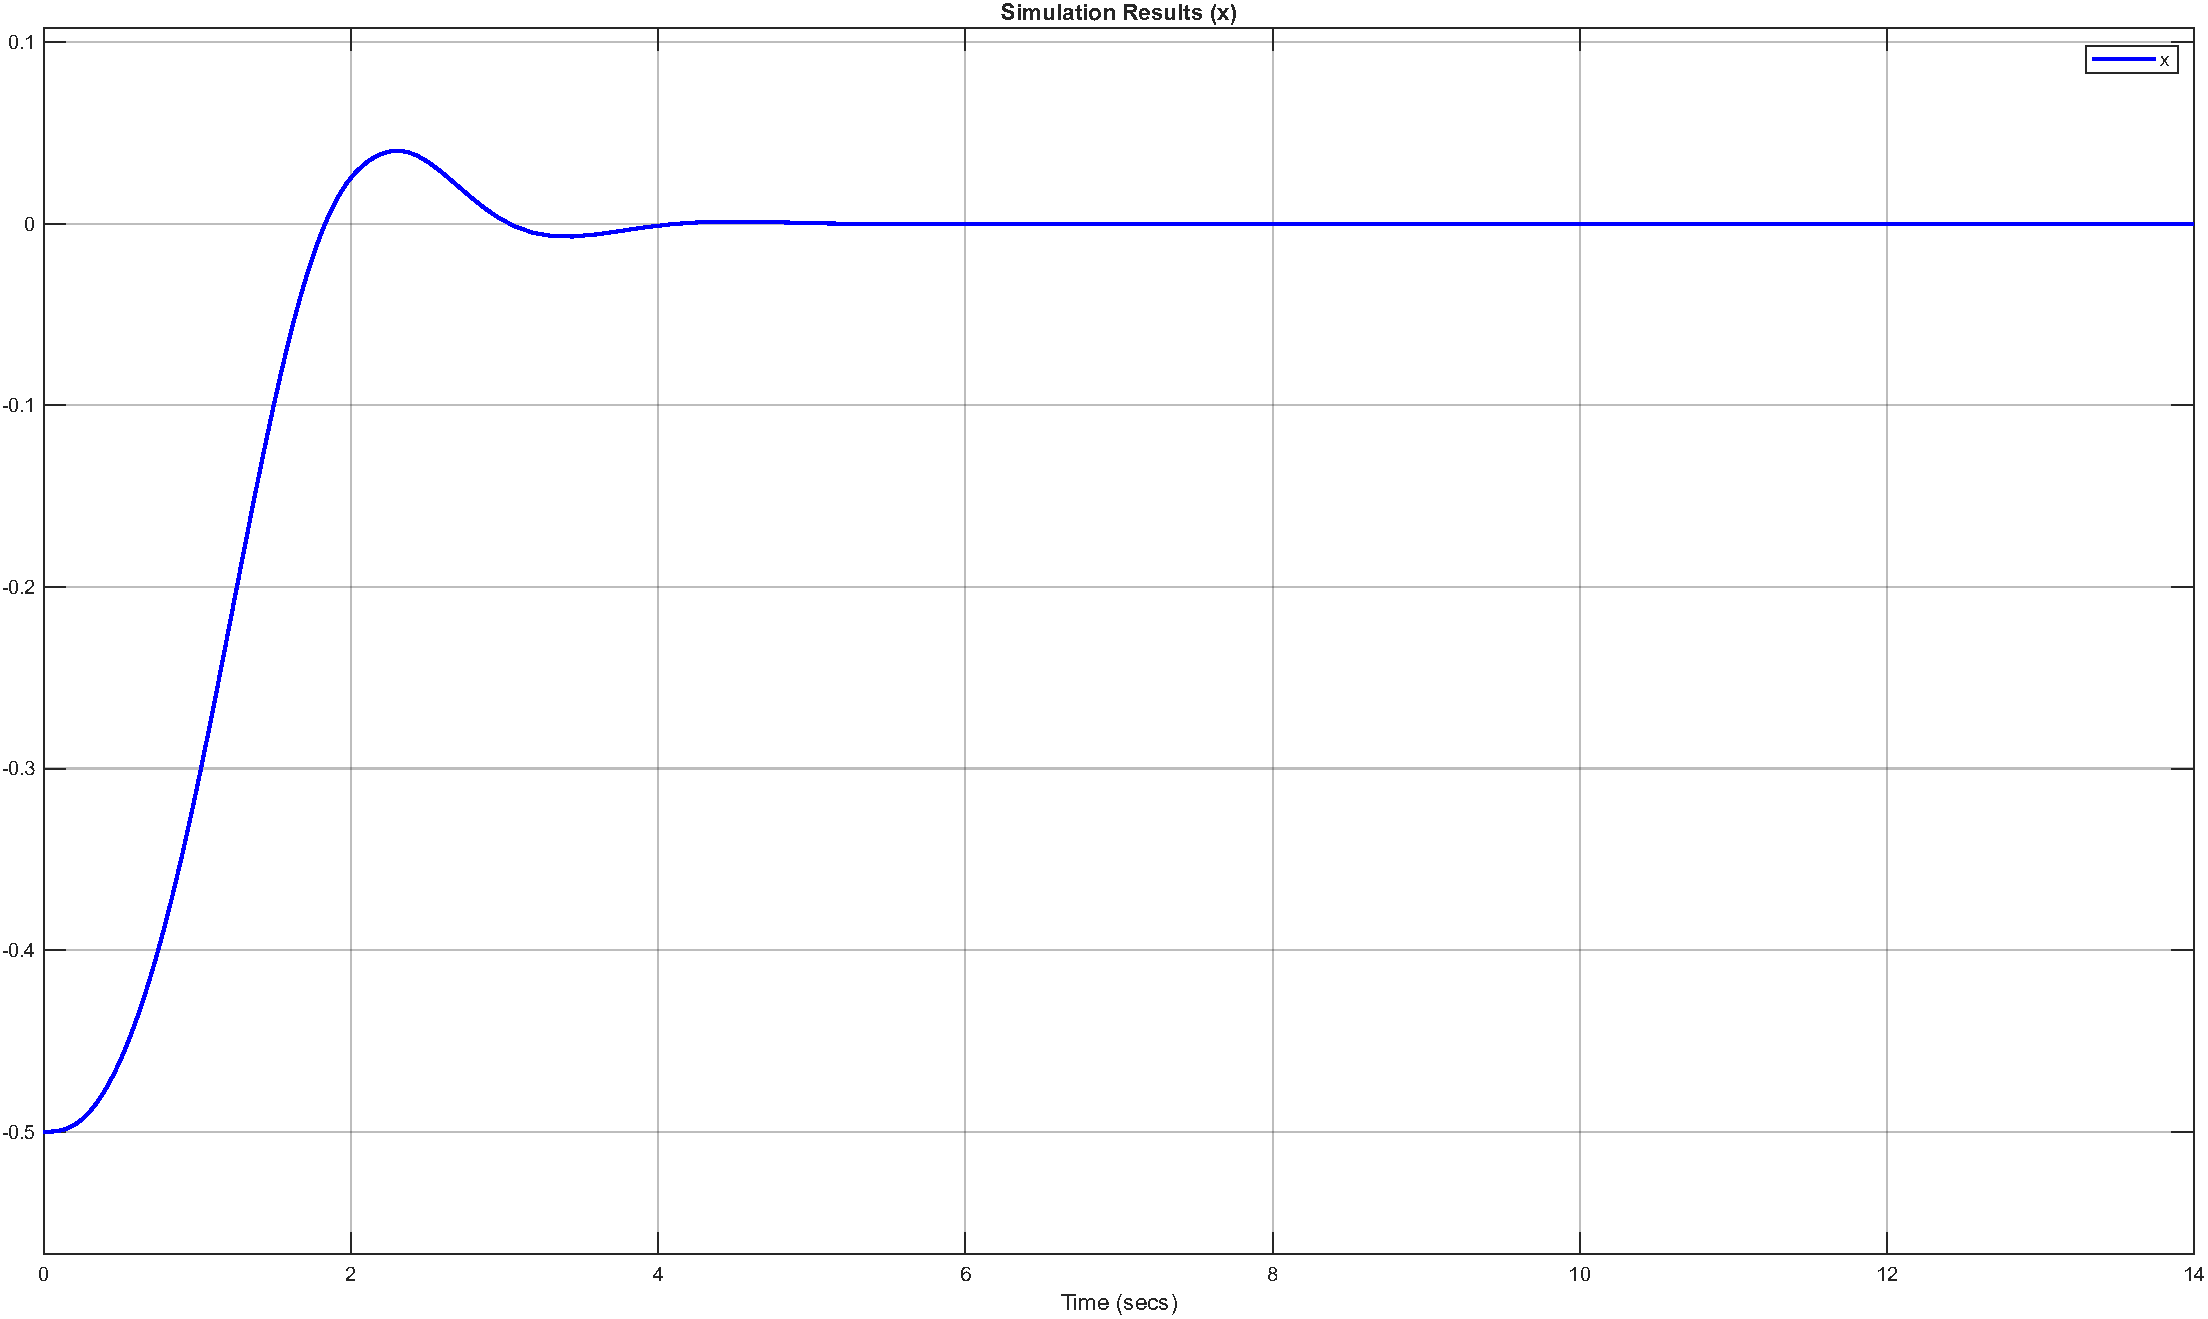
\includegraphics[width=\textwidth]{images/2_LQR_Trajectory/LQR_TRAJ_x.pdf}
        \caption{\rl{ردیابی دقیق و هموار موقعیت کالسکه در جابجایی $0.5$ متر.}}
        \label{fig:lqr_traj_x_05}
    \end{minipage}\hfill
    \begin{minipage}{0.48\textwidth}
        \centering
        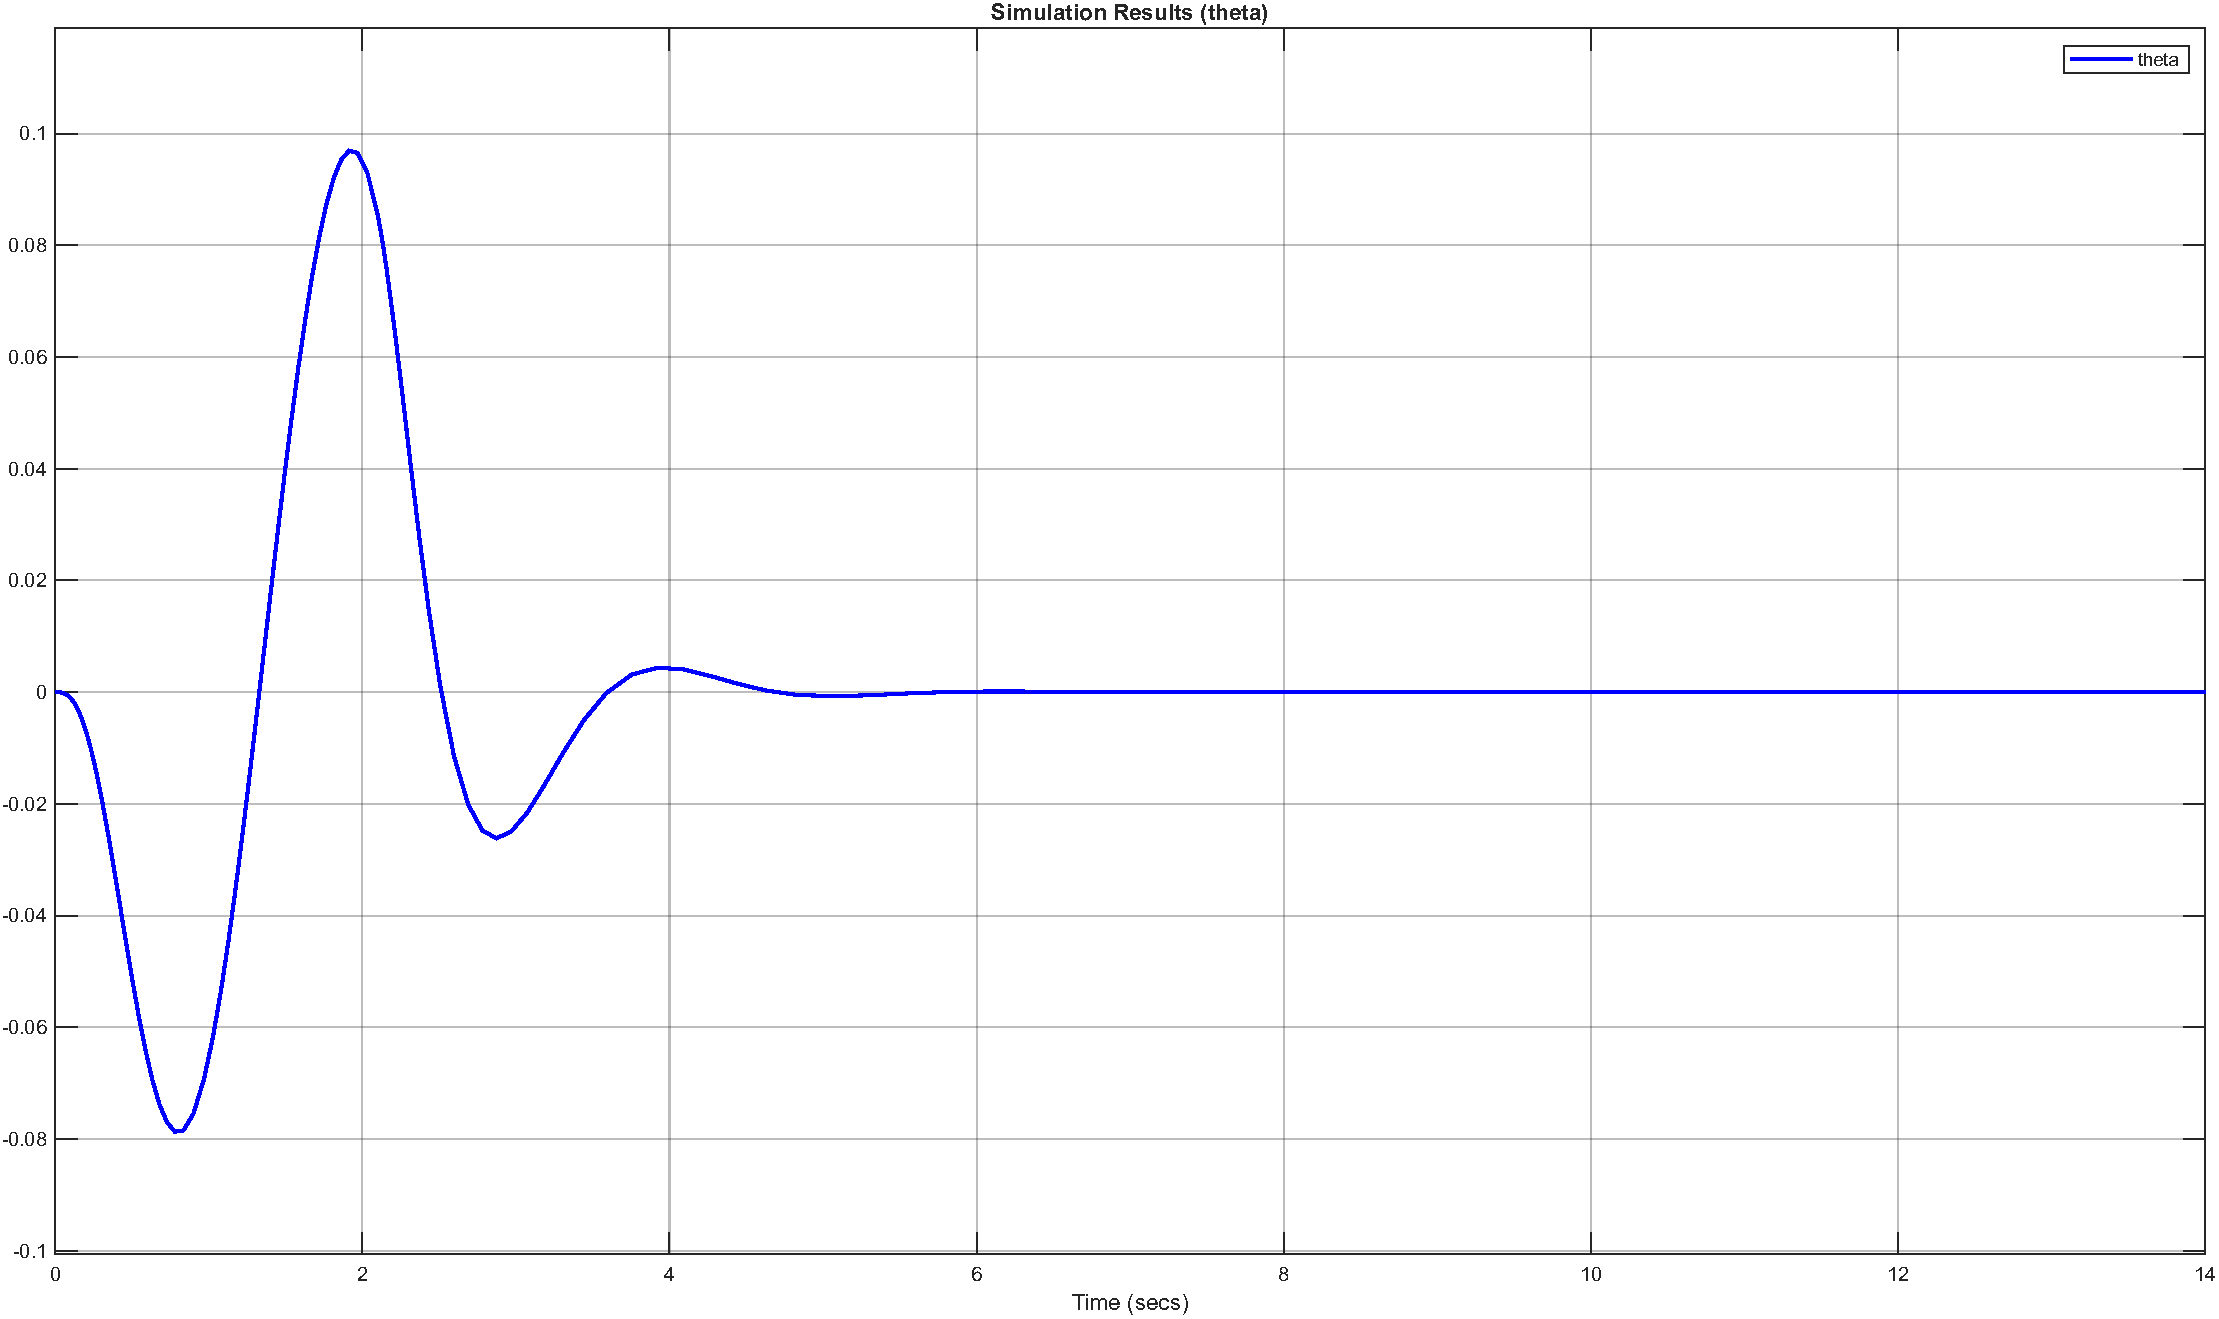
\includegraphics[width=\textwidth]{images/2_LQR_Trajectory/LQR_TRAJ_theta.pdf}
        \caption{\rl{محدود شدن زاویه نوسان آونگ به حدود $0.1$ رادیان در جابجایی $0.5$ متر.}}
        \label{fig:lqr_traj_theta_05}
    \end{minipage}
\end{figure}

\begin{figure}[htbp]
    \centering
    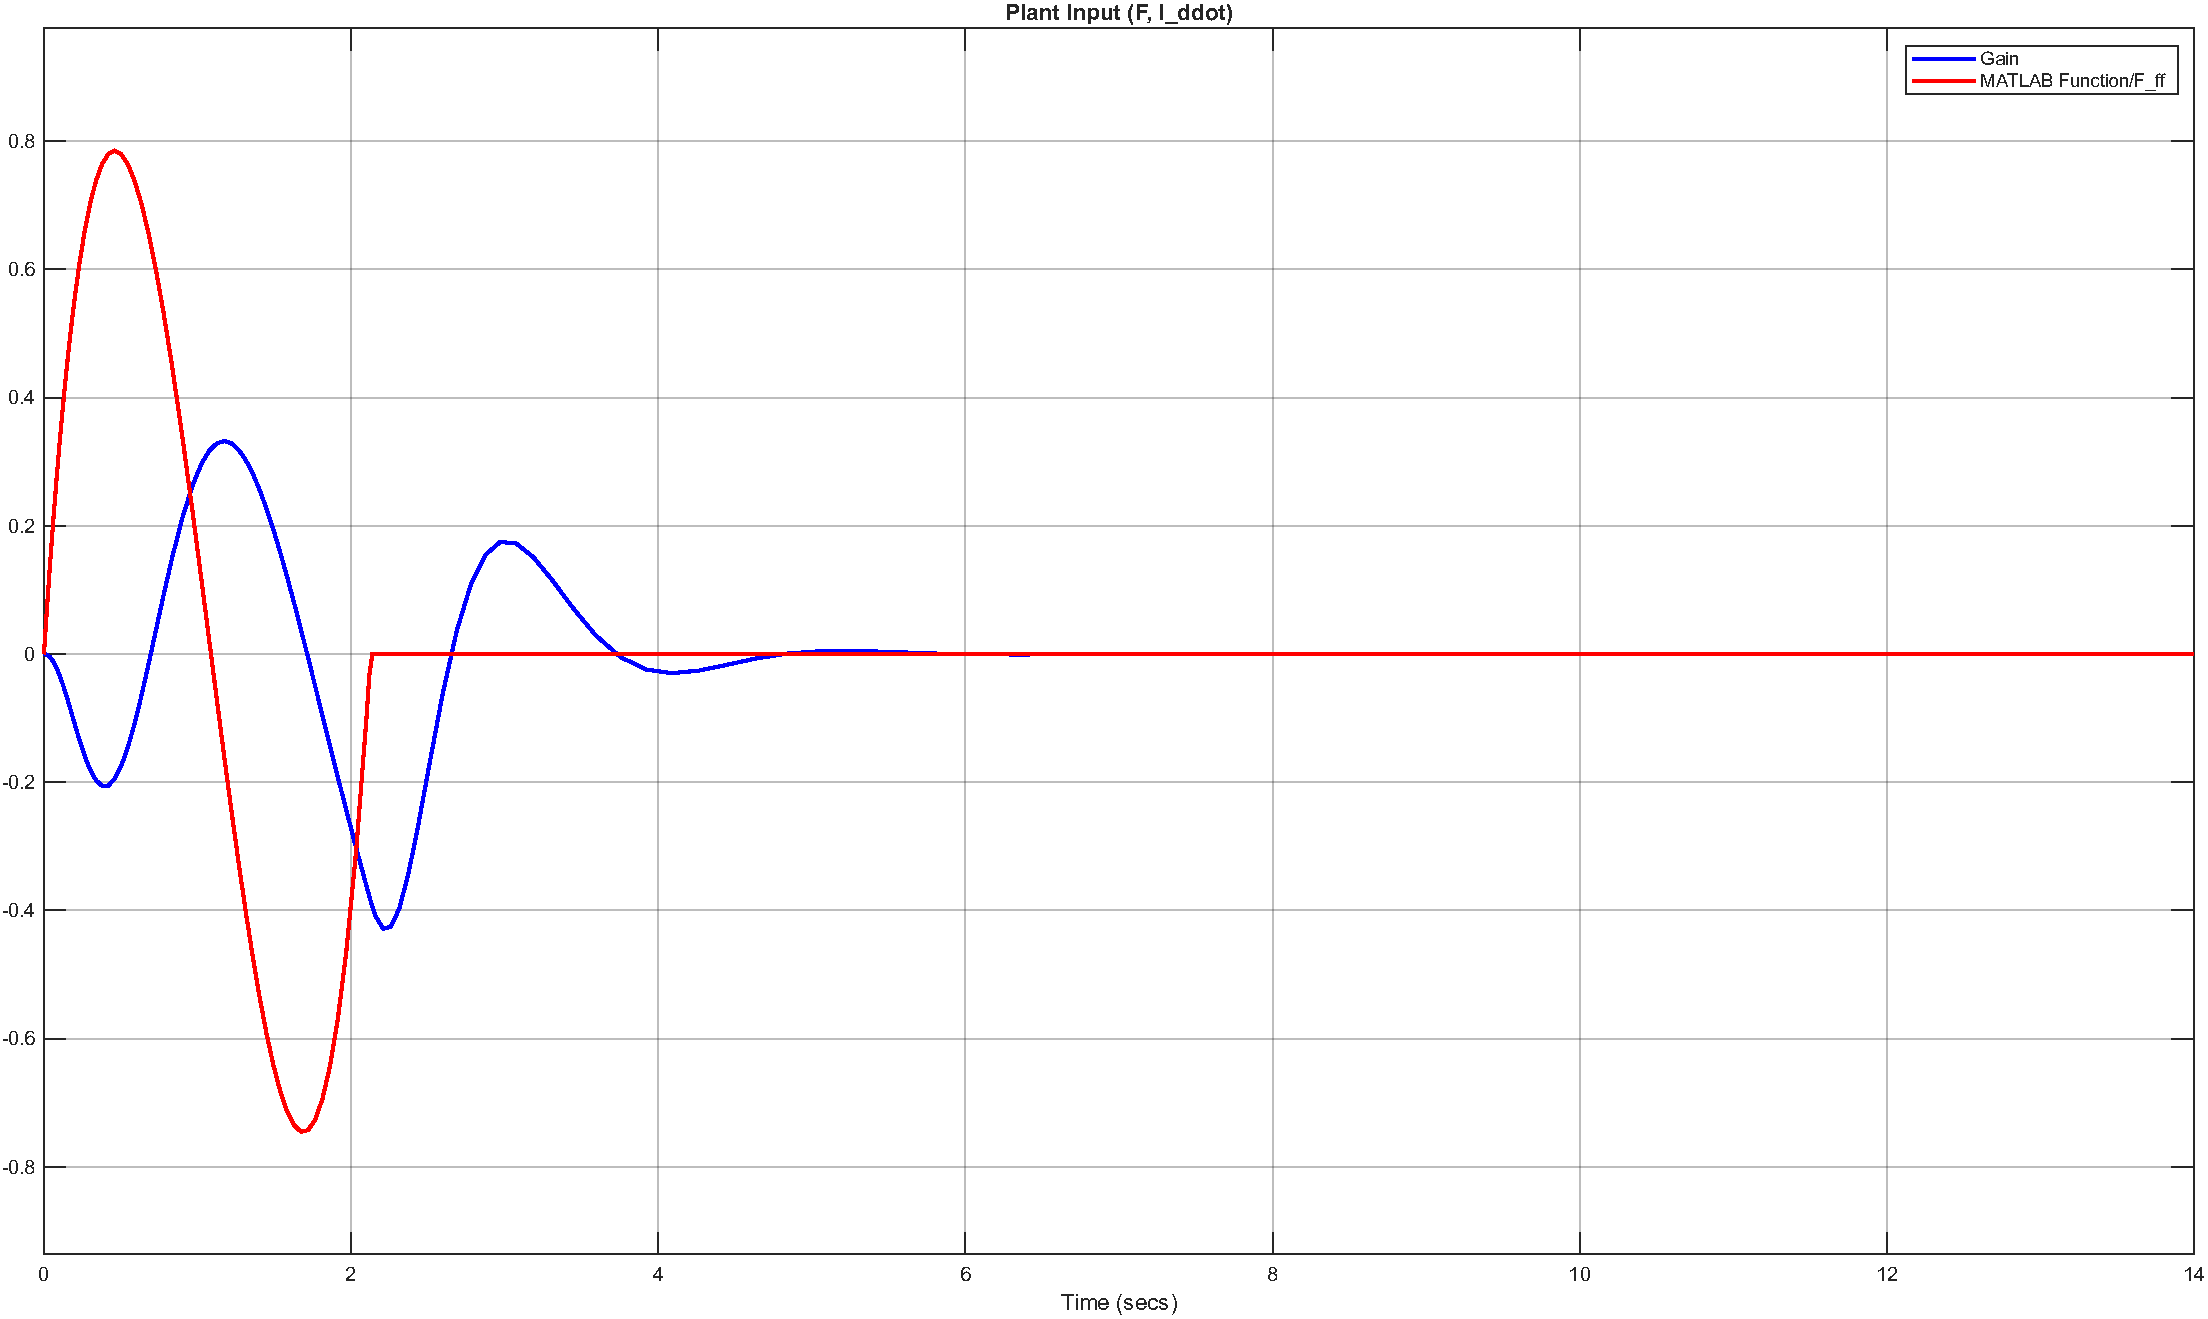
\includegraphics[width=0.6\textwidth]{images/2_LQR_Trajectory/LQR_TRAJ_Fs.pdf}
    \caption{\rl{تفکیک سیگنال‌های کنترلی (تأمین نیروی اصلی توسط فیدفوروارد و اصلاحات گذرا توسط فیدبک) در جابجایی $0.5$ متر.}}
    \label{fig:lqr_traj_fs_05}
\end{figure}

\subsection{ردیابی جابجایی بلندبرد ($5$ متر) و سینماتیک نوسان}

با تعمیم این معماری به جابجایی بزرگ $5$ متری، سیستم پایداری دینامیکی خود را به طور کامل حفظ نمود (شکل \ref{fig:lqr_traj_x_5}). این رفتار در تضاد مطلق با ناپایداری و چرخش آونگ در پاسخ پله است و کارایی برنامه‌ریز مسیر را در حفاظت از کران‌های خطی سیستم نشان می‌دهد.

مقایسهٔ رفتار نوسانی سیستم در مسیر طولانی (شکل \ref{fig:lqr_traj_theta_5}) با مسیر کوتاه پرده از یک پدیدهٔ سینماتیکی جالب برمی‌دارد: بیشینهٔ دامنهٔ نوسان در مسیر $5$ متری به حدود $0.6$ رادیان کاهش یافته است (در مقایسه با $0.1$ رادیان در مسیر $0.5$ متری). ریشهٔ فیزیکی این رفتار در منطق ریاضی برنامه‌ریز مسیر نهفته است. در مسافت‌های کوتاه، زمان کل سفر ($T$) توسط قید دینامیکی دوره تناوب آونگ (حداقل $1.5 T_p$) تعیین می‌شود که زمان نسبتاً کوتاهی است و شتاب مؤثری به کالسکه اعمال می‌کند. اما در مسافت‌های طولانی، قید حداکثر سرعت مجاز ($v_{\max}$) به گلوگاه محاسباتی تبدیل شده و زمان کل سفر را به شدت بسط می‌دهد. این کشیدگی زمان، شتاب پیکِ اعمال‌شده به کالسکه را رقیق می‌کند. از آنجا که زاویهٔ انحراف آونگ در فاز گذرا تابعی مستقیم از شتاب کالسکه است، دامنهٔ نوسان به شدت افت می‌کند.

\begin{figure}[htbp]
    \centering
    \begin{minipage}{0.48\textwidth}
        \centering
        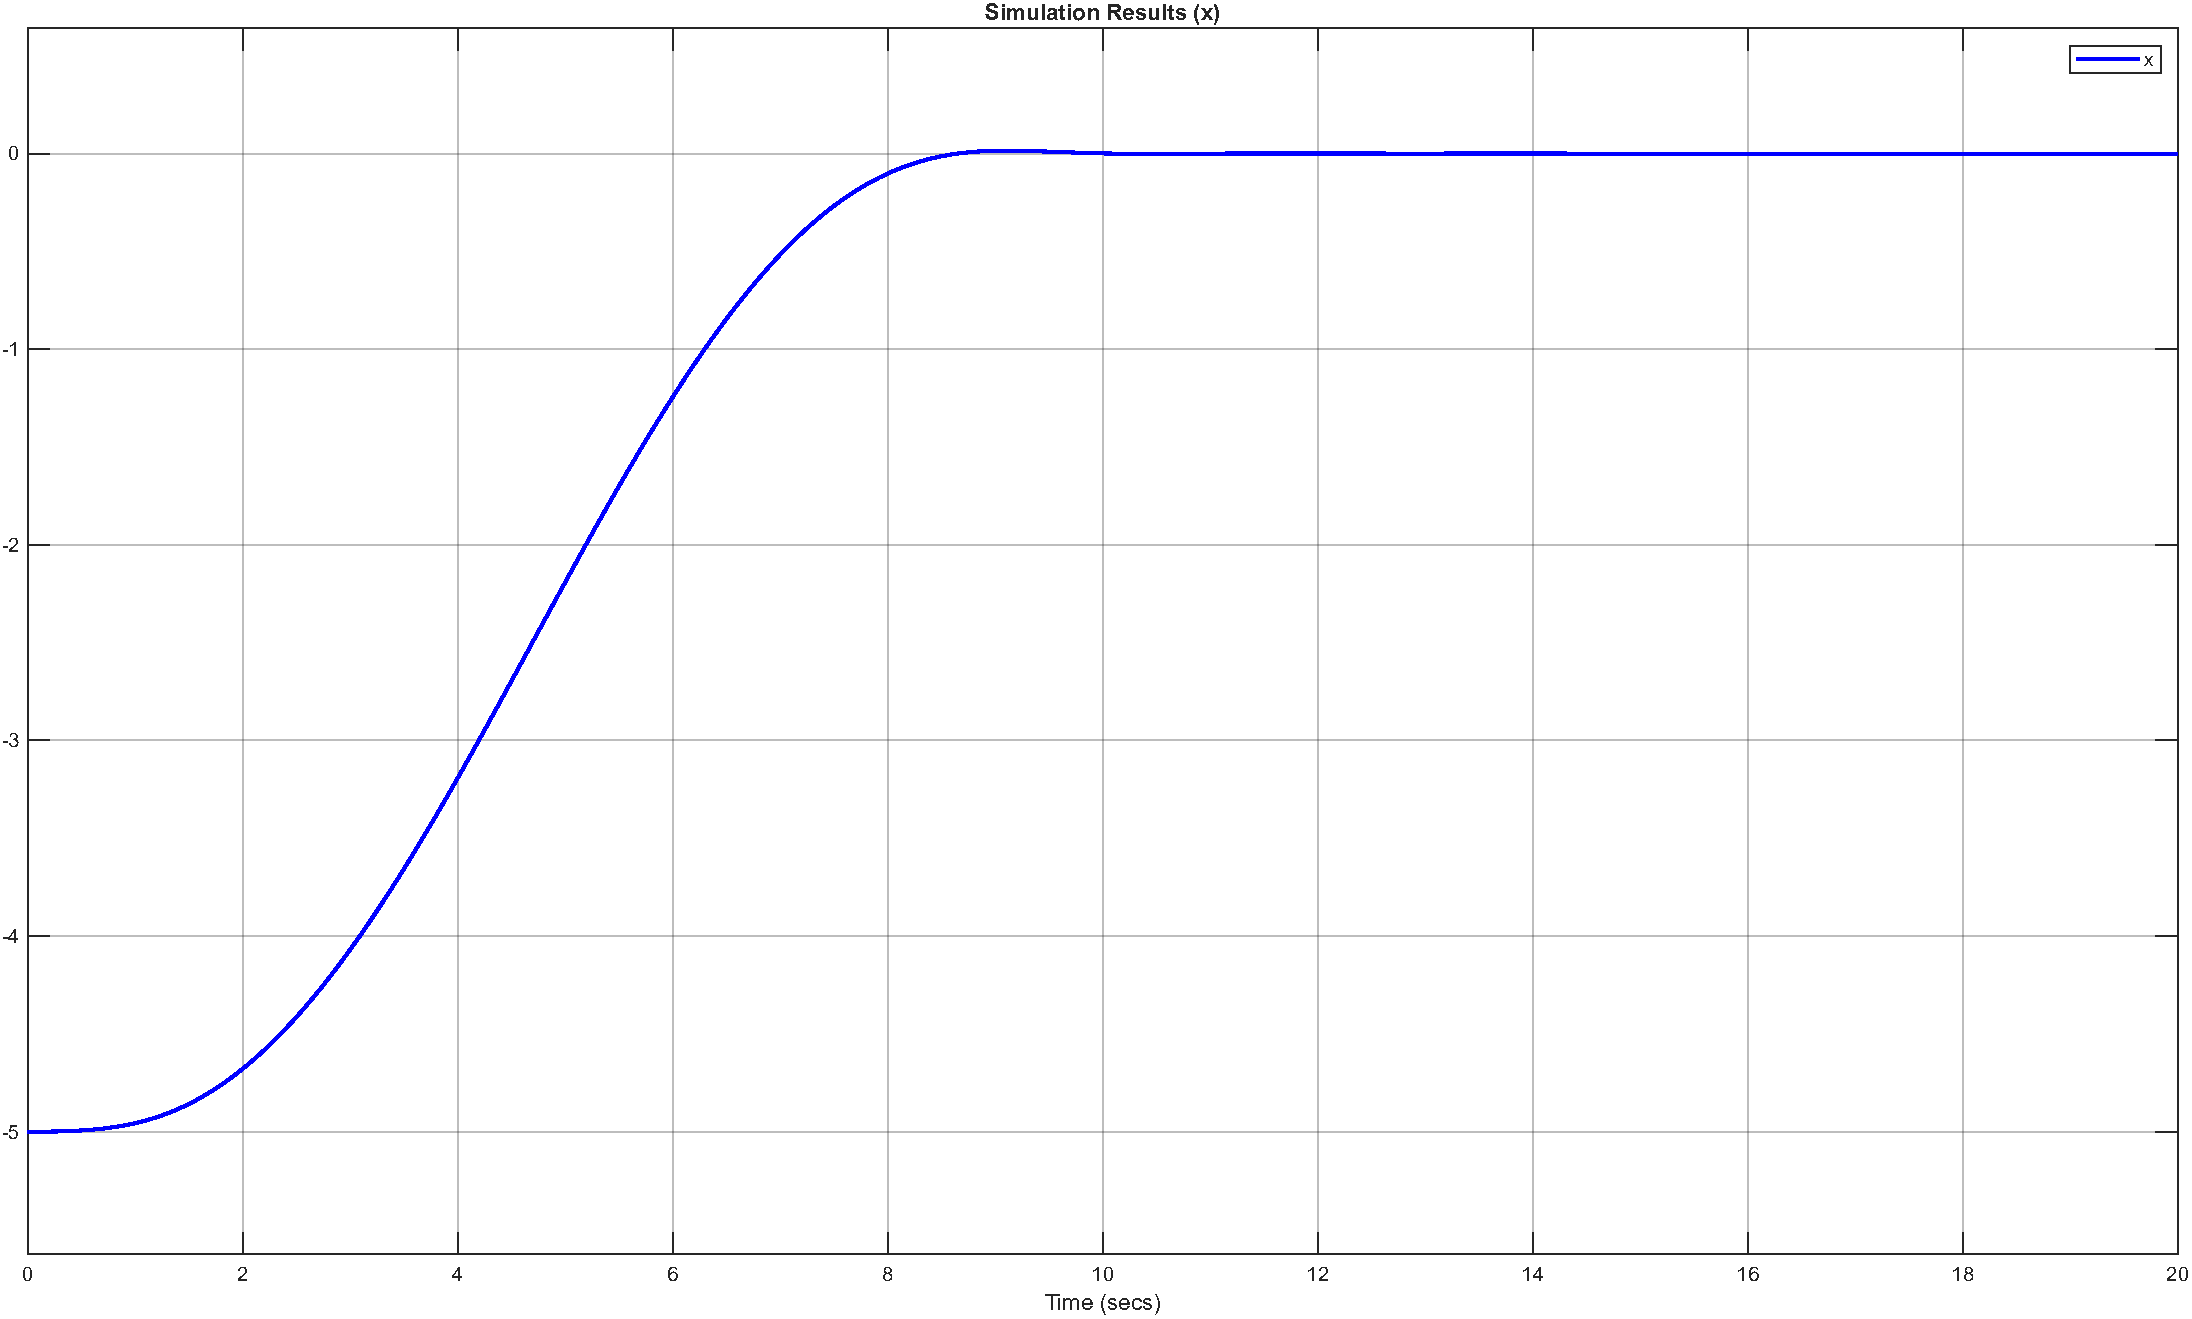
\includegraphics[width=\textwidth]{images/2_LQR_Trajectory/LQR_TRAJ_x_5.pdf}
        \caption{\rl{حفظ پایداری کامل و ردیابی موقعیت کالسکه در جابجایی بلندبرد $5$ متر.}}
        \label{fig:lqr_traj_x_5}
    \end{minipage}\hfill
    \begin{minipage}{0.48\textwidth}
        \centering
        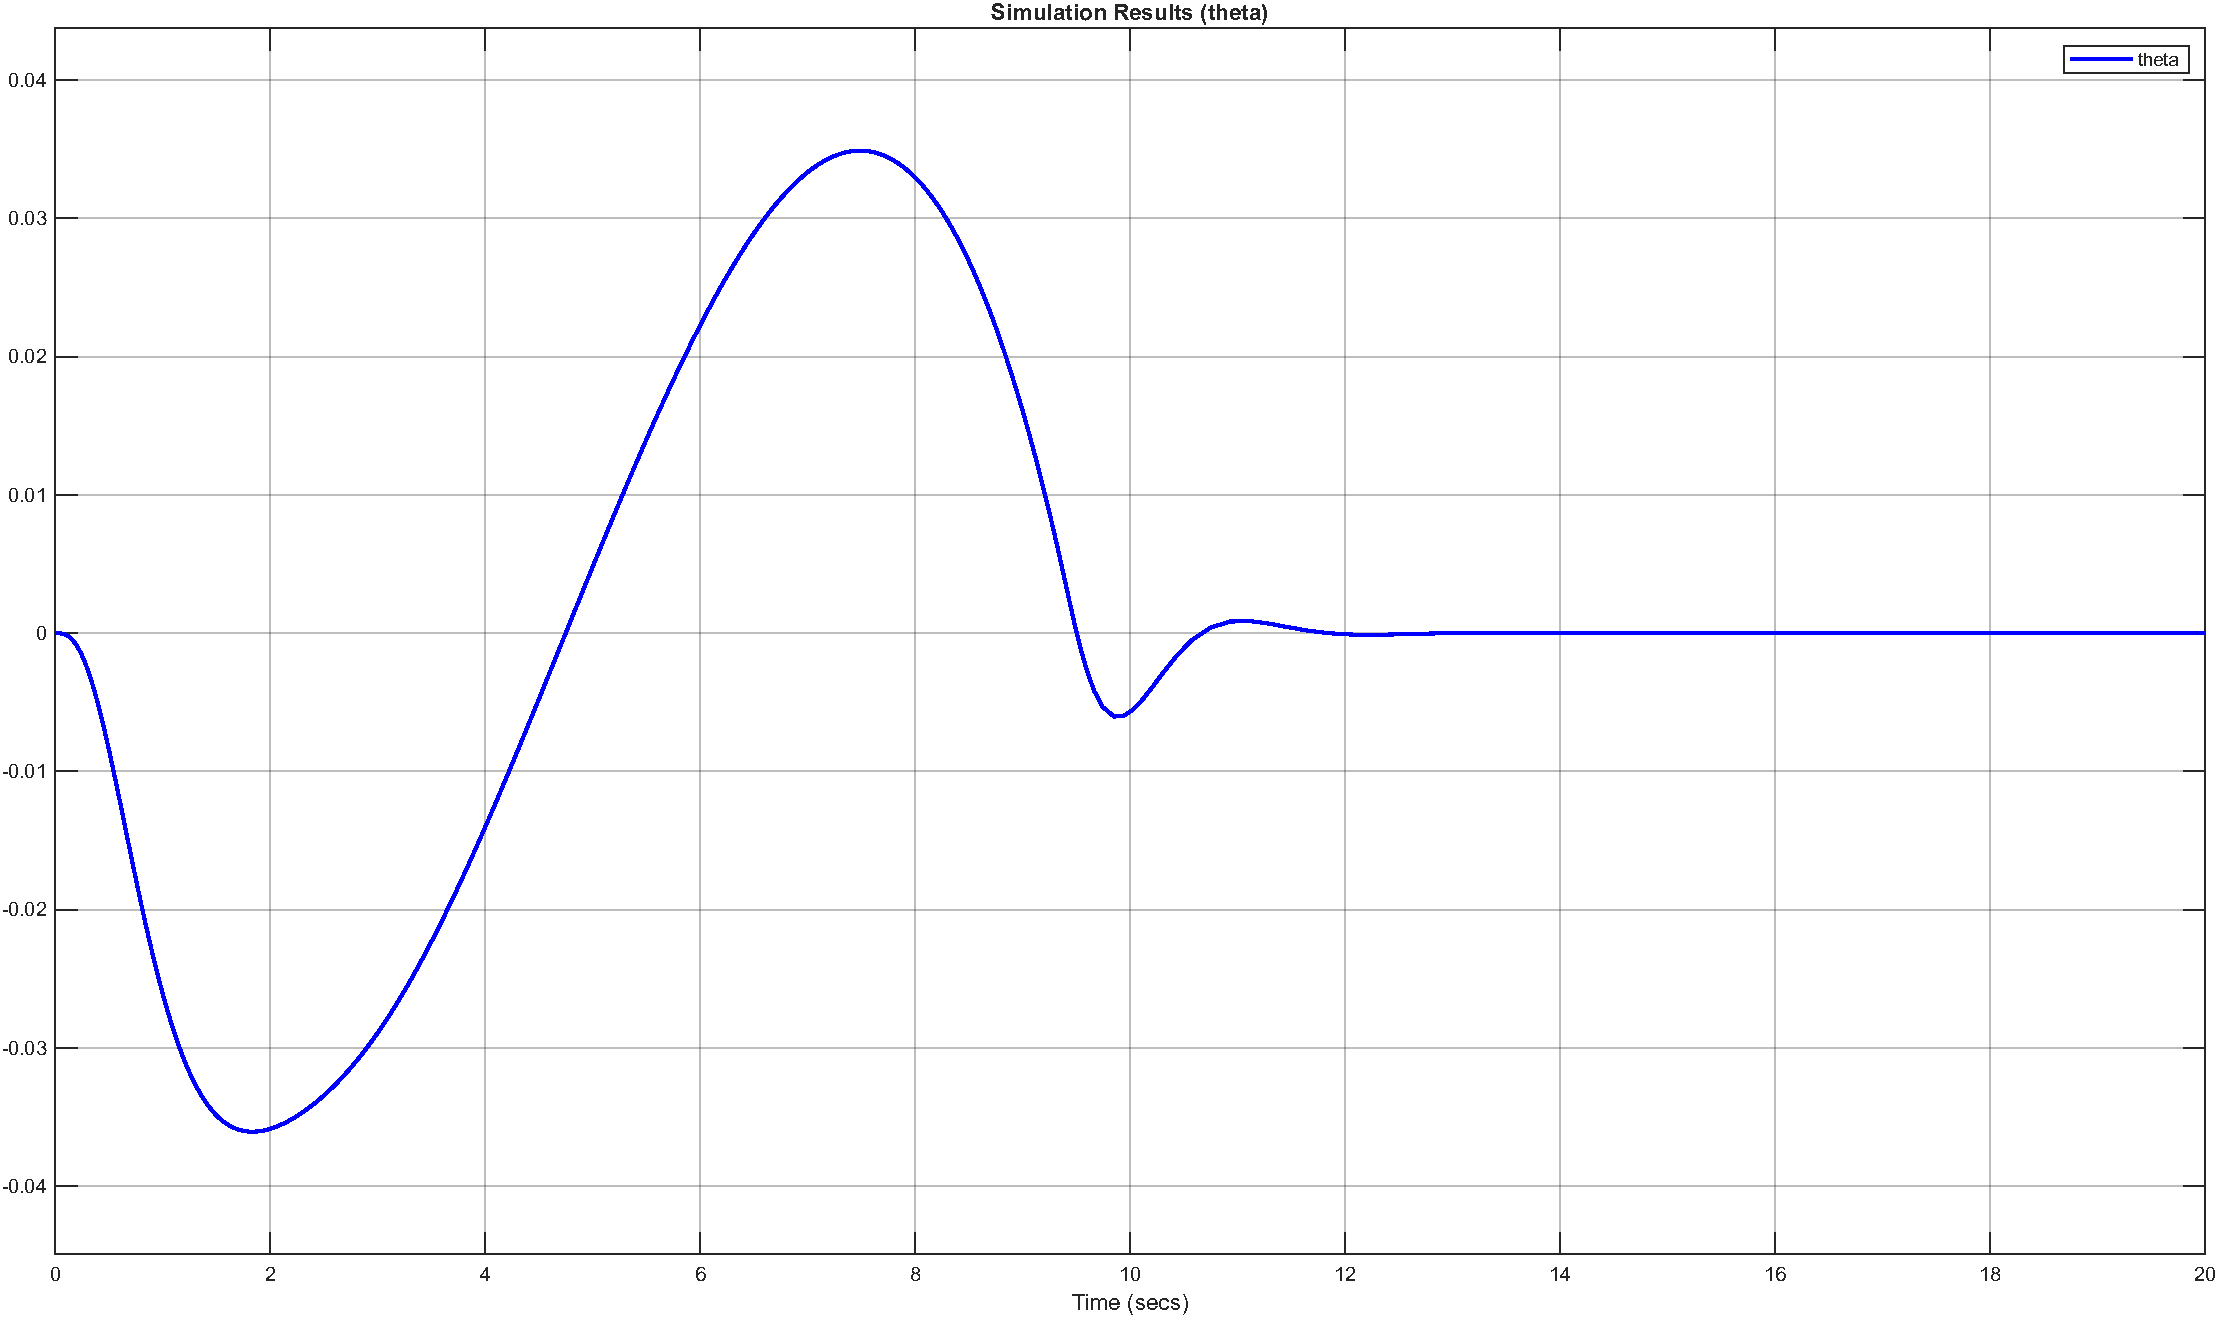
\includegraphics[width=\textwidth]{images/2_LQR_Trajectory/LQR_TRAJ_theta_5.pdf}
        \caption{\rl{کاهش دامنه نوسان به دلیل افت شتاب مؤثر و سرکوب کامل نوسانات پسماند در جابجایی $5$ متر.}}
        \label{fig:lqr_traj_theta_5}
    \end{minipage}
\end{figure}

\begin{figure}[htbp]
    \centering
    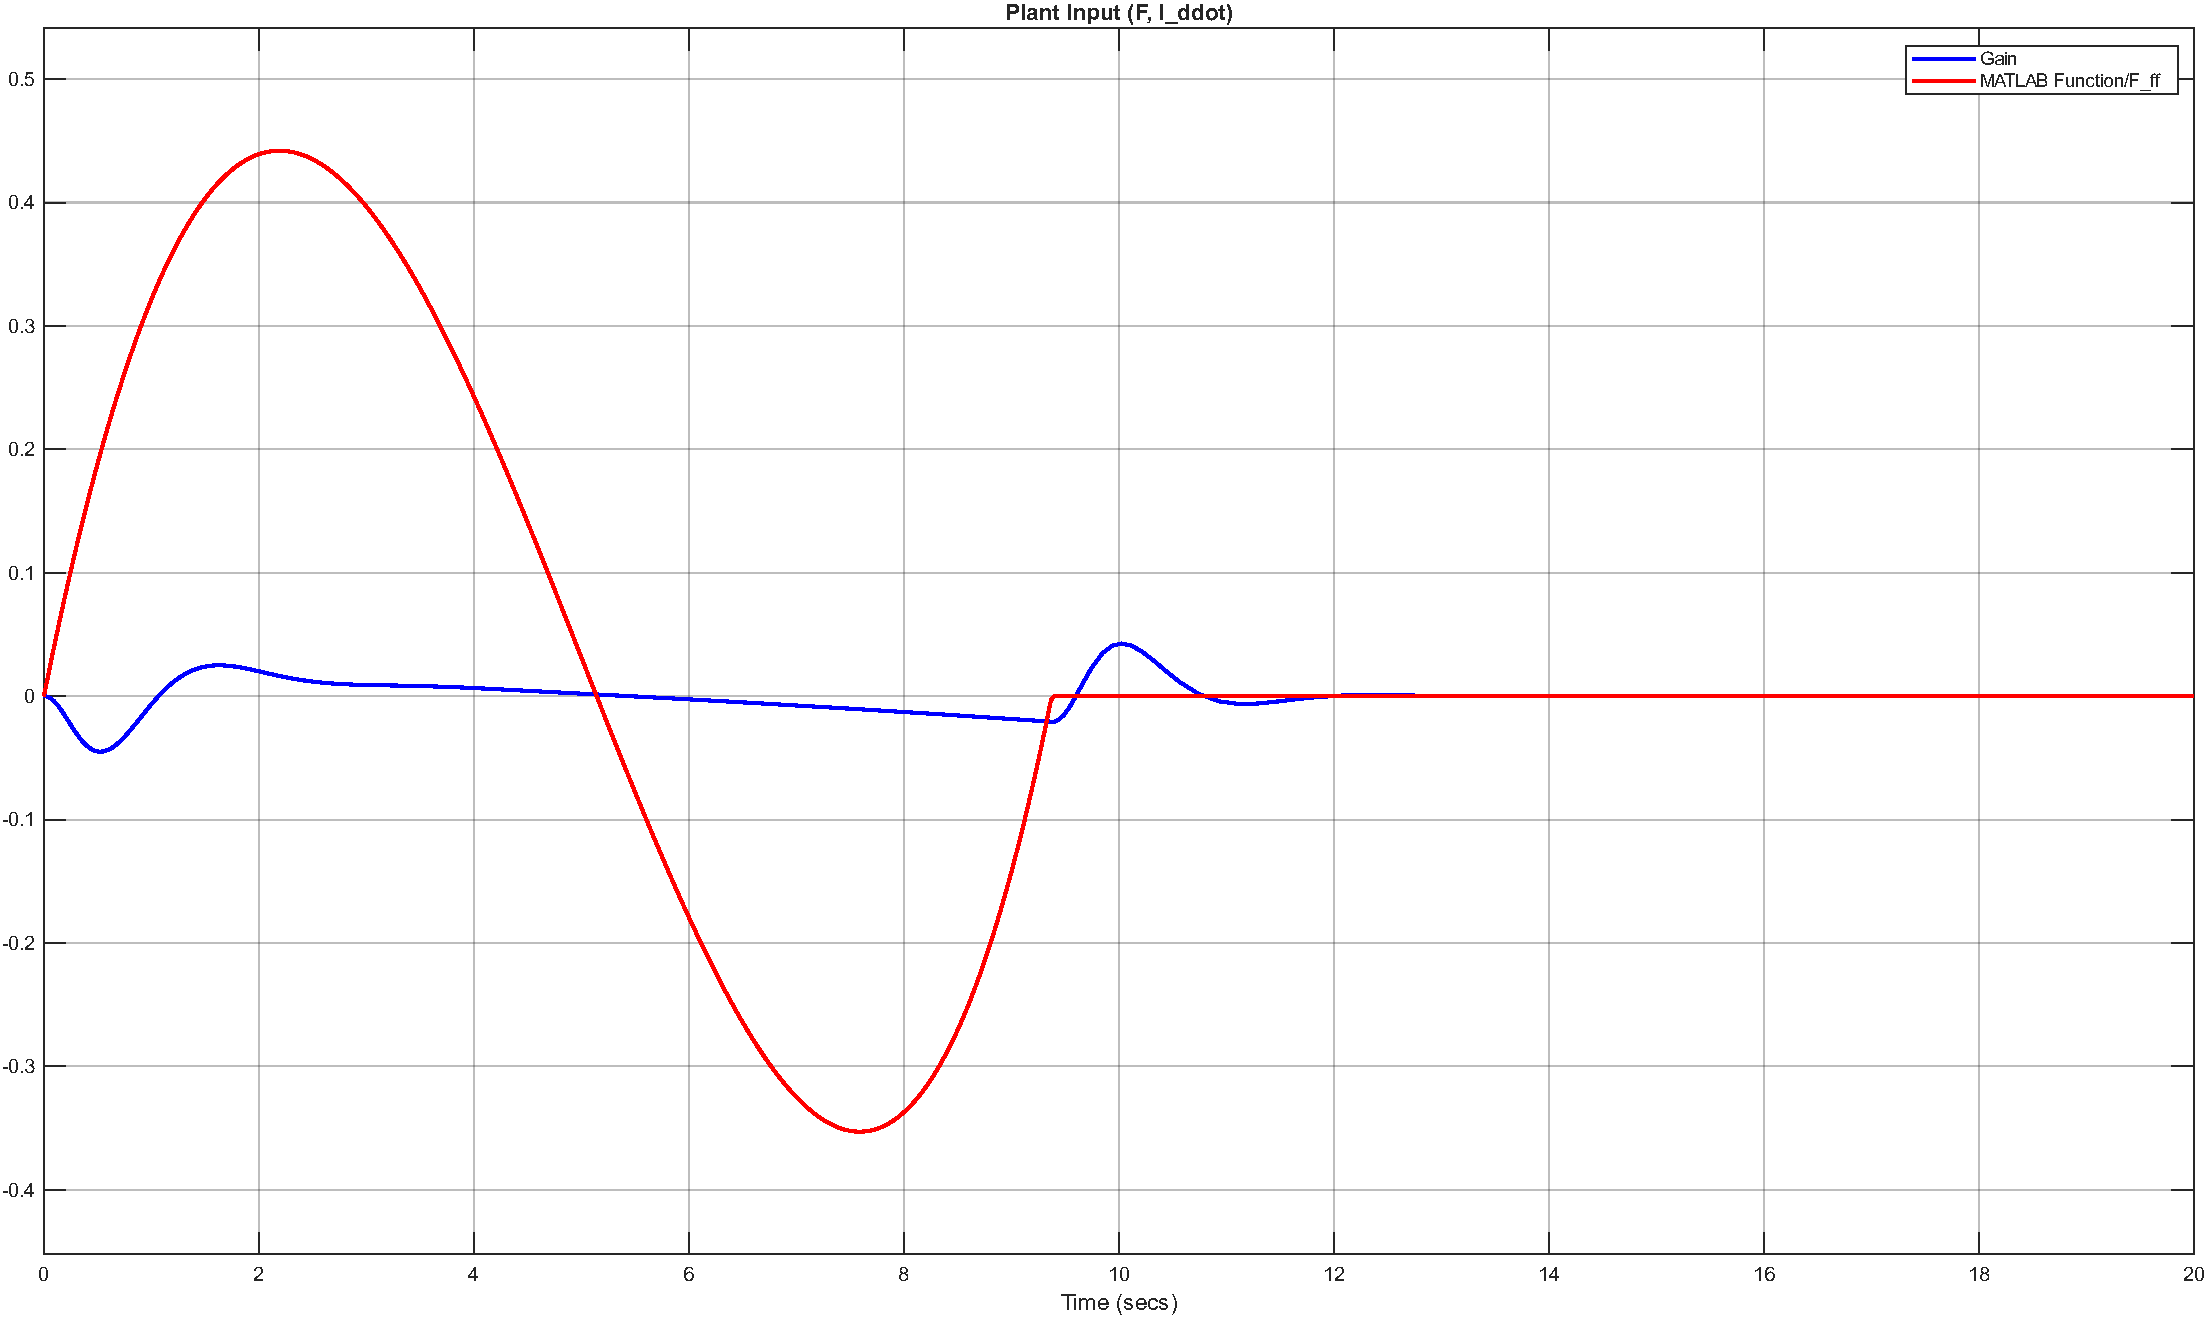
\includegraphics[width=0.6\textwidth]{images/2_LQR_Trajectory/LQR_TRAJ_Fs_5.pdf}
    \caption{\rl{پروفایل نیروی کنترلی ایمن و توزیع‌شده در زمان برای جابجایی $5$ متر.}}
    \label{fig:lqr_traj_fs_5}
\end{figure}

\subsubsection{حذف نوسانات پسماند و جمع‌بندی عملکرد \lr{LQR}}
یکی از دستاوردهای مهم معماری یکپارچهٔ \lr{LQR} و فیدفوروارد، قابلیت آن در سرکوب کامل نوسانات است. بررسی شکل \ref{fig:lqr_traj_theta_5} حاکی از آن است که پس از رسیدن کالسکه به نقطهٔ هدف (پس از ثانیهٔ $10$)، زاویهٔ آونگ به سرعت و به طور کامل به صفر میل کرده و سیستم در حالت سکون مطلق قرار می‌گیرد. کنترل‌کنندهٔ خطی توانسته است بدون نیاز به متغیر کردن طول کابل و تنها با اعمال نیروهای ظریف و دقیق جبرانی در لحظات پایانی (شکل \ref{fig:lqr_traj_fs_5})، انرژی باقیمانده در سیستم زیرفعال را تخلیه کند.

در مجموع، تحلیل‌ها اثبات می‌کنند که بهره‌گیری از یک کنترل‌کنندهٔ کلاسیک در کنار برنامه‌ریز مسیر، راهکاری کاملاً موفق، پایدار و بدون نوسان پسماند برای هدایت سیستم‌های جرثقیل سقفی در سناریوهای استاندارد است.